\documentclass{article}
\usepackage{listings}
\usepackage[utf8x]{inputenc}
\usepackage[greek=nohyphenation,english=nohyphenation]{hyphsubst}
\usepackage[greek,english]{babel}
\usepackage{geometry}
%\usepackage{showframe} 
\newgeometry{vmargin={25mm}, hmargin={25mm,25mm}}
\usepackage{graphicx}
\graphicspath{ {./images/} }


\title{Numerical Analysis Project Report}
\author{Parmenion Charistos [3173]}
\date{December 2020}

\begin{document}
\maketitle

\section*{Introduction}
This report refers to a mandatory project for the Numerical Analysis course given by the Aristotle university of Thessaloniki. Per exercise, adequate explanation and Matlab code snippets are provided. However, prerequisite knowledge on the subject is essential for its substantial comprehension.
\section{Part One}
The first task involves the plotting of the following function;
\[f(x) = e^(\sin(x)^3) + x^6 - 2x^4 - x^3 - 1\]
This is easily achieved via the \emph{plot} command in the suggested interval;
\begin{lstlisting}[language=Matlab]
x = -2:0.1:2;      
plot(x,f(x));       

function y = f(x)
    y = exp(sin(x).^3) + x.^6 - 2*x.^4 - x.^3 - 1;
end
\end{lstlisting}
\begin{figure}[h]
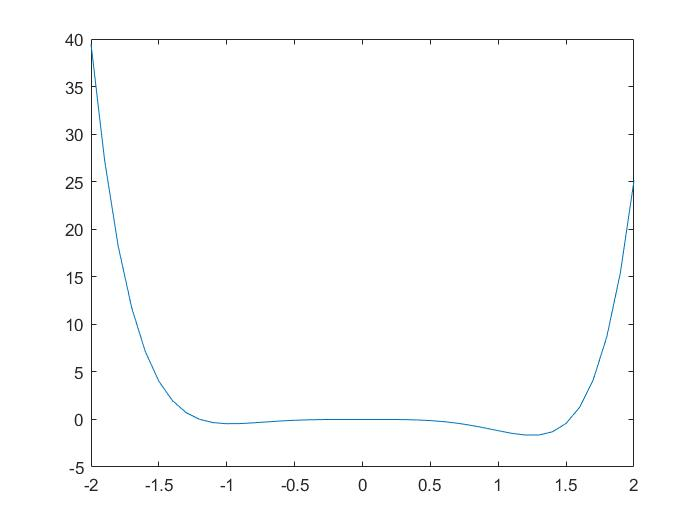
\includegraphics[scale=0.4]{images/f_plot.jpg}
\centering
\end{figure}
Afterwards, the objective is to approximate $f(x) = 0$ in the interval $[-2,2]$ using three methods. Namely, the bisection, Newton-Raphson and secant methods.
\pagebreak
\subsection{Bisection Method}
For the bisection method, the standard algorithm is executed as shown below;
\begin{lstlisting}[language=Matlab]
function root = Bisection(e,a,b)
    N = ceil(log((b-a)/e)/log(2));   %Number of iterations required.
    solved = true;

    for i = 1:N         %Implementing bisection algorithm.
       m = (a+b)/2;
       if f(m) == 0
           root = m;
           break;
       end
       if f(m)*f(a) < 0
           b = m;
       else
           if f(m)*f(b) < 0
               a = m;
           else
               disp("[Bisection Method] Not a valid interval [a,b]."); 
               disp("Initial product f(a)*f(b) should be < 0.");
               solved = false;
               break;
           end
       end
       root = m;
    end
    
    if solved
        fprintf("[Bisection Method] - Result: \n\n")   
        fprintf("Iterations: %d\n",N)                
        fprintf("Root: %.5f\n",root)                 
        fprintf("f(%.5f) = %.15f\n",root,f(root)) 
    end
end
\end{lstlisting}
The \emph{Bisection} function takes as parameters the maximum desired error \emph{e} one needs to achieve and the bounds of the interval $[a,b]$. For the method to work, the $a,b$ parameters should fulfil the Bolzano's theorem's condition; \[f(a)f(b)<0\]It, then, calculates the required number of iterations N, using the known error-based formula and proceeds to approximate the initial equation's solution by continuously dividing the interval $[a,b]$ in two. Meanwhile, the algorithm picks the half that continues to fulfil the Bolzano condition, until the remaining interval, which contains at least one root for the equation, is narrow enough for the error to be within its set limits.\\*\\*For the current example, the Bolzano condition is met for $a = -1, b = 2$. Hence, the following function call;
\begin{lstlisting}[language=Matlab]
Bisection(e,-1,2);
\end{lstlisting}
The result of the previous function call (5-digit precision);
\begin{lstlisting}
[Bisection Method] - Result: 

Iterations: 20
Root: 1.53013
\end{lstlisting}
\pagebreak
\subsection{Newton - Raphson Method}
For the Newton - Raphson method, the preconditions consist of the following;
\begin{itemize}
    \item $f(x)$ is twice differentiable in $[a,b]$
    \item $f'(x),f''(x) \neq 0, \forall x \in (a,b)$
    \item $f(x_0)f''(x_0) > 0$
\end{itemize}
The $f(x)$ function in our example is indeed twice differentiable in the given interval.\\*The first and second derivatives are defined as;
\begin{lstlisting}[language=Matlab]
%First derivative.
function y = fd(x)
    y = 3*exp(sin(x).^3)*cos(x)*sin(x).^2+6*x.^5-8*x.^3-3*x.^2;
end

%Second derivative.
function y = fdd(x)
    y = 9*exp(sin(x).^3)*cos(x).^2*sin(x).^4 - 3*exp(sin(x).^3)*sin(x).^3 
        + 6*exp(sin(x).^3)*cos(x).^2*sin(x) + 30*x.^4 - 24*x.^2 - 6*x;
end 
\end{lstlisting}
These are, then, utilized in the \emph{Newton - Raphson} function below. This function receives two parameters. The maximum error \emph{e} allowed for the root approximation and the initial $x_0$. It then proceeds to sequentially produce the next approximation, based on the previous one, until there is a difference whose absolute value is less than \emph{e}.\\*\\*This is demonstrated in the excerpt below;
\begin{lstlisting}
function root = Newton_Raphson(e,x_prev)
    N = 0;                               %Iterations counter.
    current_e = intmax;                  %Current Error (initialized as max)

    while current_e > e                  %Implementing algorithm.
        N = N+1;                                  
        x_next = x_prev - f(x_prev)/fd(x_prev);   
        root = x_next;                            
        current_e = abs(x_next - x_prev);         
        x_prev = x_next;                          
    end    

    fprintf("\n\n[Newton Raphson Method] - Result: \n\n")   
    fprintf("Iterations: %d\n",N)                
    fprintf("Root: %.5f\n",root)         
    fprintf("f(%.5f) = %.15f\n",root,f(root)) 
end
\end{lstlisting}
For the current example, the third condition concerning $x_0$ is fulfilled for $x_0=2$.\\*Hence, the function call;
\begin{lstlisting}[language=Matlab]
Newton_Raphson(e,2);
\end{lstlisting}
The result of the previous function call (5-digit precision);
\begin{lstlisting}
[Newton Raphson Method] - Result: 

Iterations: 7
Root: 1.53013
\end{lstlisting}
\pagebreak
\subsection{Secant Method}
The secant method follows the same principles with the Newton - Raphson method, yet it's particularly useful in case the first and second derivatives of the function in use cannot be easily calculated. Thus, its preconditions are the same, except it requires two initial input values $x_0, x_1$ instead of one, which are usually set as the bounds of the selected interval. Its precise function and formula are displayed below;
\begin{lstlisting}[language=Matlab]
function root = Secant(e,x_2prev,x_prev)           
    N = 0;                      %Iterations counter.
    current_e = intmax;         %Current Error (initialized as max).

    while current_e > e         %Implementing algorithm.
        N = N+1;                                                                    
        x_next = x_prev - (f(x_prev)*(x_prev - x_2prev))/(f(x_prev) - f(x_2prev));  
        root = x_next;                                                              
        current_e = abs(x_next - x_prev);                                           
        x_2prev = x_prev;
        x_prev = x_next;                                                            
    end    

    fprintf("\n\n[Secant Method] - Result: \n\n")   
    fprintf("Iterations: %d\n",N)                
    fprintf("Root: %.5f\n",root) 
    fprintf("f(%.5f) = %.15f\n",root,f(root)) 
end
\end{lstlisting}
The \emph{Secant} method does not directly use the derivatives of the function in use, yet it computes its root's approximation in an almost identical manner as the Newton - Raphson. By setting $x_0=-2, x_1=2$, the following function call outputs the according results;
\begin{lstlisting}[language=Matlab]
Secant(e,-2,2);
\end{lstlisting}
Output;
\begin{lstlisting}
[Secant Method] - Result: 

Iterations: 11
Root: 1.53013
\end{lstlisting}
\pagebreak
\subsection{Newton - Raphson Convergence}
In the previous sections, three algorithms that use numerical approximation were examined.
\\*Their parameters were set in order to compare their efficiency when targeting the
same root. It is obvious that, when viable, the Newton - Raphson method achieves the
same precision in the fewest iterations. Following, is the secant method, which
adopts the same philosophy. Last, is the far simpler bisection method.
\\*\\*This is indeed, the ranking iterations-wise when all three methods can be
applied on the same problem. However, one must select the most suitable option,
considering the total computational cost per algorithm, which may or may not include
e.g. the calculation of the function's derivatives.
\\*\\*In the current example, there existed a few more roots in the given interval,
which can be approximated if the functions' input parameters are tweaked
accordingly. These are given in the following vector;\[[-1.19762, 0, 1.53013]\]The methods' efficiency comparison does not differ in those cases.
\\*\\*The Newton - Raphson method is known for its quadratic convergence, which is based on
the fixed - point theory, meaning that the square of the error at one iteration is
proportional to the error at the next iteration. This is the case in the current example as
well. However, there are a few exceptions which cause this method not to converge (quadratically or at all);
\begin{itemize}
    \item $f'(x_n)=0$ at some iteration (causes division by zero)
    \item $x_0$ is set too far from the actual root
    \item the function used is hyperbolically convex (causes divergence towards infinity)
\end{itemize}
\pagebreak
\section{Part Two}
The next task is to modify the previous methods in accordance to some basic instructions. In detail;
\begin{enumerate}
    \item The bisection method now picks a random point \emph{m} within the interval $[a,b]$ of the previous iteration.
    \item The Newton - Raphson method has a new formula that also utilizes $f''(x)$.
    \item The secant method now uses three values $x_0,x_1,x_2$ in its new formula. Hence, the next term is dependent on the previous two.
\end{enumerate}
Then, apply them to solve $f(x)=0$ for a new function;
\begin{lstlisting}[language=Matlab]
%--f function--
function y = f(x)
    y = 94*cos(x).^3 - 24*cos(x) + 177*sin(x).^2 - 108*sin(x).^4
        - 72*cos(x).^3 * sin(x).^2 - 65;
end

%--f' function--
function y = fd(x)
    y = (216*cos(x).^2 - 432*cos(x))*sin(x).^3
        + (-144*cos(x).^4 - 282*cos(x).^2 +354*cos(x) + 24) * sin(x);
end

%--f'' function--
function y = fdd(x)
    y = (432 - 432*cos(x))*sin(x).^4 + (1224*cos(x).^3 - 1296*cos(x).^2 
        + 564*cos(x) - 354)*sin(x).^2 - 144*cos(x).^5 
        - 282*cos(x).^3 + 354*cos(x).^2 + 24*cos(x);
end
\end{lstlisting}
\pagebreak
\subsection{Modified Bisection Method}
For the bisection method, the modification is quite simple. The only change is the manner in which $m$ is calculated, which now adopts a value generated by the \emph{rand} command within the interval $(a,b)$.
\\*\\*This, however, causes a further minor change, since, now, the number of iterations N cannot be calculated precisely beforehand. Thus, a while - loop is used, which runs until the next approximation differs less than \emph{e}, in absolute value, than the previous one.
\\*\\*The code is otherwise identical;
\begin{lstlisting}[language=Matlab]
function root = Mod_Bisection(e,a,b)
    N = 0;                           %Iterations counter.
    current_e = intmax;
    solved = true;

    while current_e > e
       N = N + 1;
       m = a + (b - a).*rand;        %New formula.
       if f(m)*f(a) < 0
           b = m;
       else
           if f(m)*f(b) < 0
               a = m;
           else
               disp("[Modified Bisection Method] Not a valid interval [a,b].");
               disp("Initial product f(a)*f(b) should be < 0.");
               solved = false;
               break;
           end
       end
       current_e = abs(b-a);
       root = m;
    end

    if solved
        fprintf("\n\n[Modified Bisection Method] - Result: \n\n")   
        fprintf("Iterations: %d\n",N)                
        fprintf("Root: %.5f\n",root)     
        fprintf("f(%.5f) = %.15f\n",root,f(root)) 
    end
end
\end{lstlisting}
Using this method on the new function, the following root was approximated;
\begin{lstlisting}[language=Matlab]
Mod_Bisection(e,0,3);

[Modified Bisection Method] - Result: 

Iterations: 17
Root: 0.84107
\end{lstlisting}
\pagebreak
\subsection{Modified Newton - Raphson Method}
For the Newton - Raphson, the only alteration made, occurred for the formula of the next approximation's calculation. It now also directly utilizes the second derivative of the function in use, which is expected to improve the accuracy per approximation and thus, reduce the iterations required.
\\*\\*The function is identical with the original except for the line below, which updates the formula;
\begin{lstlisting}[language=Matlab]
x_next = x_prev - f(x_prev)/fd(x_prev) 
         - ((f(x_prev).^2).*fdd(x_prev))/(2*(fd(x_prev).^3));
\end{lstlisting}
By implementing this method we got the following output;
\begin{lstlisting}
Mod_Newton_Raphson(e,1);

[Modified Newton Raphson Method] - Result: 

Iterations: 15
Root: 1.04719
\end{lstlisting}
\subsection{Modified Secant Method}
Except for the new formula and the afore mentioned extra parameter, the secant method did undergo any other substantial change. It is, thus, given by the following;
\begin{lstlisting}[language=Matlab]
function root = Mod_Secant(e,x0,x1,x2)
    N = 0;                      %Iterations counter.
    current_e = intmax;         %Current Error (initialized as max)

    while current_e > e
        N = N+1;                        %Incrementing iterations.
        q = f(x0)/f(x1);
        r = f(x2)/f(x1);
        s = f(x2)/f(x0);
        %New formula.
        x3 = x2 - (r*(r-q)*(x2 - x1) + (1-r)*s*(x2 - x0))/((q-1)*(r-1)*(s-1));  
        root = x3;                      %Updating current approximation.
        current_e = abs(x3 - x0);       %Updating error after iteration.                                                                                 
        x2 = x1;
        x1 = x0;
        x0 = x3;
    end    

    fprintf("\n\n[Modified Secant Method Result]: \n\n")   
    fprintf("Iterations: %d\n",N)                
    fprintf("Root: %.5f\n",root) 
    fprintf("f(%.5f) = %.15f\n",root,f(root)) 
end
\end{lstlisting}
An example of this method's output is given below;
\begin{lstlisting}
Mod_Secant(e,1,1.5,0);

[Modified Secant Method Result]: 

Iterations: 26
Root: 1.04719
\end{lstlisting}
\pagebreak
\subsection{Analysis}
A few of the function's roots have been displayed as examples above, yet there are a few more which can be approximated, given the appropriate tweaking of the methods' input parameters. These are given in the following vector;\[[0.84107, 1.04719, 2.30052]\]
\\*As per request, the modified bisection method was run consecutively ten times in the interval $[-1,2]$.
\\*The results, as expected, showed that the method does not converge within a fixed number of iterations. Actually, for the same root, with common input parameters, the iterations of convergence varied from 17 to 32, an impressive difference in efficiency.
\\*\\*What followed was the comparison of the original methods with their modified equivalents. First, a common interval and input parameters were set for each couple of methods under examination, with the exception of the modified secant method which receives an extra parameter by default. Then, each duo underwent some thorough testing to conclude the following;
\begin{itemize}
    \item[--]The bisection method is steady and reliable, although it does not converge in fewest iterations. 
    \item[--]The modified bisection is unreliable and  performs worse than the original, apart from very few exceptions.
    \item[--]The modified Newton - Raphson converges in fewer iterations than the original, yet it seems more sensitive to diverge outwards of the desired interval.
    \item[--]The modified secant method achieves greater or equal performance to the original, based on how close the initial parameters are to the root.
\end{itemize}
\pagebreak
\section{Part Three}
In this section, the task involved the design of three algorithms that concern linear equations systems. Namely, an algorithm that solves a system of the sort $\mathbf{Ax = b}$ via $\mathbf{PA = LU}$ analysis, an algorithm that calculates the Cholesky decomposition of a matrix $A$ and an algorithm that approximates a system's solution vector using the Gauss - Seidel method. These are displayed in the corresponding order below;
\subsection{PA = LU Analysis}
The theory behind this method is described as follows. For a system of the sort $\mathbf{Ax = b}$, the matrix $\mathbf{A}$ can be analyzed into a product $\mathbf{LU}$, where $\mathbf{L}$ is a lower triangular matrix with $\mathbf{1}$s on its main diagonal and $\mathbf{U}$ is an upper triangular matrix.
\\*\\*However, before forming the product, $\mathbf{A}$ must undergo some optimization changes, as in switching its rows, which are depicted by the permutation matrix $\mathbf{P}$. By the end of this procedure, the initial system can be substituted to adopt the form of $\mathbf{LUx = Pb}$.
\\*\\*Then, what remains to calculate the solution vector $\mathbf{x}$ is to solve two simple systems. $\mathbf{Ly = r}$, where $\mathbf{y = Ux}$ and $\mathbf{r = Pb}$, and subsequently $\mathbf{Ux = y}$.
\\*\\*This is exactly what the following functions accomplish;
\begin{lstlisting}[language=Matlab]
function [P,A,L,U,x] = SolveSystem(A,b)
    n = size(A,1);                      
    [A,P] = SortDrivers(A);     %Sort A and form permutation matrix P.
    [L,U] = LU_Analysis(A);     %Calculate matrices L*U = A.
    r = P*b;                    %Rename P*b product (for ease of use).
    
    %We now have a system of the form LUx = r.
    %Let y = Ux.
    
    y(1) = r(1)/L(1,1);         %Solve Ly = r for y.
    for i=2:1:n
        sum = 0;
        for j=1:1:i-1
           sum = sum+L(i,j)*y(j); 
        end
        y(i) = (r(i)-sum)/L(i,i);
    end
    
    x(n) = y(n)/U(n,n);         %Solve Ux = y for x.
    for i=n-1:-1:1
        sum=0;
        for j=n:-1:i
            sum = sum+U(i,j)*x(j);
        end
        x(i) = (y(i)-sum)/U(i,i);
    end
    x = transpose(x);
end
\end{lstlisting}
\pagebreak
The \emph{SolveSystem} function receives as parameters the matrix of coefficients $\mathbf{A}$ and the column vector of constants $\mathbf{b}$ and proceeds to solve the system, once it has retrieved the $\mathbf{P,L,U}$ matrices from the other helper functions.
\\*\\*The \emph{SortDrivers} function receives a matrix $\mathbf{A}$ as a parameter and proceeds to sort its each
main diagonal, in order for each driver element to have a greater absolute value than the elements below it
which belong in the same column. This is achieved by finding the max element by absolute value per column
and switching the matrix' rows accordingly.
\\*\\*The procedure is executed via the following snippet;
\begin{lstlisting}[language=Matlab]
function [A,P] = SortDrivers(A)
    n = size(A,1);
    P = zeros(n,n);
    
    for i=1:1:n
        P(i,i) = 1;  %Create n-Identity matrix P.
    end
    
    for j=1:1:n
        max = 0;
        optimal_row = j;
        for i=j:1:n                 %For each column:        
            if abs(A(i,j)) > max    %Find element with max abs.
                max = abs(A(i,j));  %Update max.
                optimal_row = i;    %Save index of row that contains max.
            end
        end
        if j ~= optimal_row   %If max is not a driver element, swap rows.
            A([j optimal_row],:) = A([optimal_row j],:);
            P([j optimal_row],:) = P([optimal_row j],:);
        end
    end
end
\end{lstlisting}
\pagebreak
The last function used is the \emph{LU Analysis} function. This receives a matrix $\mathbf{A}$ as its parameter and calculates the matrices $\mathbf{LU}$, for which $\mathbf{PA = LU}$ is true. For its design, the classic LU analysis algorithm was used, extracted from the "Introduction to Numerical Analysis" book of Akrivis and Dougalis and is presented as follows;
\begin{lstlisting}
function [L,U] = LU_Analysis(A)       
    n = size(A,1);
    U = zeros(n,n);
    L = zeros(n,n);
    for i=1:1:n         %Using the classic LU analysis algorithm.
        for j=1:1:i-1
            sum = 0;
            for k=1:1:j-1
                sum = sum + L(i,k)*U(k,j);
            end
            L(i,j) = (A(i,j) - sum) / U(j,j);
        end
        L(i,i) = 1;
        for j=i:1:n
            sum = 0;
            for k=1:1:i-1
                sum = sum + L(i,k)*U(k,j);
            end
            U(i,j) = A(i,j) - sum;
        end
    end
end
\end{lstlisting}
\subsection{Cholesky Decomposition}
For this section the widespread Cholesky algorithm was used, which efficiently produces the Cholesky Decomposition of a positive, symmetric matrix. The algorithm was extracted from the "Introduction to Numerical Analysis" book of Akrivis and Dougalis and is described by the following;
\begin{lstlisting}
function L = Cholesky(A)
    n = size(A,1);
    for i=1:1:n     %Using the classic Cholesky decomposition algorithm.
       for j=1:1:i-1
           sum = 0; 
           for k=1:1:j-1
                sum = sum + L(i,k)*L(j,k);
           end
           L(i,j) = (A(i,j)-sum) / L(j,j);
       end
       
       sum = 0;
       for k=1:1:i-1
           sum = sum + L(i,k)^2;
       end
       L(i,i) = sqrt(A(i,i) - sum);
    end
end
\end{lstlisting}
The \emph{Cholesky} function receives a matrix $\mathbf{A}$ as a parameter and is used to obtain a matrix $\mathbf{L}$ for which the following is true;
\[\mathbf{LL^\top = A}\]
\subsection{Gauss - Seidel}
For this task, an algotithm was designed which approximates the solution vector $\mathbf{x}$ of a linear equations system, using the Gauss - Seidel method. The classic algorithm was used to design the following function;
\begin{lstlisting}[language=Matlab]
function [x,N] = Gauss_Seidel(n,e)
    %Defining n-n tridiagonal matrix A. 
    A = zeros(n,n);      
    
    for i = 1:1:n
       A(i,i) = 5;
       A(i+1,i) = -2;
       A(i,i+1) = -2;
       b(i) = 1;
    end

    b(1) = 3;             %Defining vector of constants b.
    b(end) = 3;
    b = transpose(b);
    
    x = zeros(n,1);       %Defining vector x0.
    norm = 0;             %Initializing infinity norm of x0;
    N = 0;                %Iterations counter.
    
    current_e = intmax;
    x_next = zeros(n,1);  %Initializing next-approximation vector.
    
    while current_e > e
        N = N + 1;
        for i=1:1:n       %Using classic Gauss-Seidel algorithm.
            sum1 = 0;
            for j=1:1:i-1
                sum1 = sum1 + A(i,j)*x_next(j);
            end
            
            sum2 = 0;
            for j=i+1:1:n
                sum2 = sum2 + A(i,j)*x(j);
            end
               
            x_next(i) = (1/A(i,i))*(b(i) - sum1 - sum2);   %Updating sequence.
        
        norm_next = 0;
        for k=1:1:n                         %Calculating new infinity norm.
            if abs(x_next(k)) > norm_next
                norm_next = abs(x_next(k));
            end
        end
        
        current_e = norm_next - norm;   %Updating current error.
        x = x_next;                     %Saving current approximation vector.
        norm = norm_next;          %and its norm for the following iteration.
    end
end
\end{lstlisting}
\pagebreak
The $\mathbf{Gauss - Seidel}$ function, takes as a parameter the dimension \emph{n} and the maximum desired error \emph{e} and proceeds to create a \emph{n-n} tridiagonal matrix $\mathbf{A}$ with the specified elements on its diagonals.
\\*\\*Then, the standard algorithm is applied where the next approximation of the solution vector $\mathbf{x}$ is calculated via the two sums taking place in the algorithm, until the absolute difference of two consecutive approximations falls lower than \emph{e}.
\section{Part Four}
\subsection{Is stochastic?}
It is known that a square \emph{n-n} matrix $\mathbf{P}$, which contains non negative elements $p_{ij}$ and for which the following is true;
\[\sum_{j} p_{ij} = 1, (i=1,2,...)\]
is stochastic and a Markov's chain transition matrix.
\\*\\*In our current example, the $\mathbf{G}$ matrix is known to contain non negative elements, as well as it is known that the sum of each column equals $\mathbf{1}$. Hence, since the $\mathbf{G}$ matrix fulfils the entirety of the afore mentioned preconditions, it comprises a stochastic matrix.
\subsection{Maximum Eigenvector of G}
In this section, the task involved constructing the $\mathbf{G}$ matrix and calculating the eigenvector of its maximum eigenvalue, using the power method. This was accomplished through the following short script;
\begin{lstlisting}[language=Matlab]
A = [0 1 0 0 0 0 0 0 1 0 0 0 0 0 0;     %Defining matrix A.
     0 0 1 0 1 0 1 0 0 0 0 0 0 0 0;
     0 1 0 0 0 1 0 1 0 0 0 0 0 0 0;
     0 0 1 0 0 0 0 0 0 0 0 1 0 0 0;
     1 0 0 0 0 0 0 0 0 1 0 0 0 0 0;
     0 0 0 0 0 0 0 0 0 1 1 0 0 0 0;
     0 0 0 0 0 0 0 0 0 1 1 0 0 0 0;
     0 0 0 1 0 0 0 0 0 0 1 0 0 0 0;
     0 0 0 0 1 1 0 0 0 1 0 0 0 0 0;
     0 0 0 0 0 0 0 0 0 0 0 0 1 0 0;
     0 0 0 0 0 0 0 0 0 0 0 0 0 0 1;
     0 0 0 0 0 0 1 1 0 0 1 0 0 0 0;
     0 0 0 0 0 0 0 0 1 0 0 0 0 1 0;
     0 0 0 0 0 0 0 0 0 1 1 0 1 0 1;
     0 0 0 0 0 0 0 0 0 0 0 1 0 1 0];
 
 A = transpose(A);  
 
 n = size(A,1);     %Setting n.
 q = 0.15;          %Setting q.
 G = zeros(n,n);    %Initializing Google matrix.
 
 S = zeros(n,1);    %Calculating sums of columns of matrix A.
 for i=1:1:n
    for j=1:1:n
        S(i) = S(i) + A(j,i);
    end
 end
 
 for i=1:1:n        %Defining Google matrix (according to formula).
     for j=1:1:n 
         G(i,j) = q/n + (A(i,j)*(1-q))/S(j);
     end
 end
\end{lstlisting}
By this point, the $\mathbf{G}$ matrix is formed and can, thus, be used as a parameter for the power method, described in the following \emph{Power Method} function;
\begin{lstlisting}[language=Matlab]
function lambda = Power_Method(G)
    n = size(G,1);
    b = rand(n,1); %Generating random column-vector b.
    
    for i=1:1:n    %Implementing algorithm.
        b_next = G*b;
        j = 1;
        while b(j) == 0
            j = j + 1;
        end
        b_next = (1/b_next(j)) * b_next;
        b = b_next;
    end
    
    sum = 0;     %Calculating sum of elements of calculated eigenvector.
    for i=1:1:n
        sum = sum + b(i);
    end
    
    lambda = (1/sum) * b;  %Normalizing eigenvector.
 end
\end{lstlisting}
This function generates a random column vector $\mathbf{b}$ of length \emph{n} and proceeds to apply the power method, repeating the procedure \emph{n} times, as instructed in order to reach the max eigenvalue and hence its according eigenvector. The result is then normalized for its elements to add up to $\mathbf{1}$, since they refer to probabilities. The output provided, when the result is printed is;
\[[0.0268,0.0299,0.0299,0.0268,0.0396,0.0396,0.0396,0.0396,0.0746,0.1063,0.1063,0.0746,0.1251,0.1163,0.1251]\]
which confirms the given data.
\pagebreak
\subsection{Page Rank Modification}
For this task, four new links were added in the original $\mathbf{A}$ matrix and two were removed, aiming to improve the rank of page 15. In detail, links from page 15 were added to pages 9,10,12,13 and links from pages 3 and 8 were removed. The new matrix $\mathbf{A}$ now has the following form;
\begin{lstlisting} [language = Matlab]
A =  [0 1 0 0 0 0 0 0 1 0 0 0 0 0 0;
      0 0 1 0 1 0 1 0 0 0 0 0 0 0 0; 
      0 1 0 0 0 1 0 0 0 0 0 0 0 0 0;  
      0 0 1 0 0 0 0 0 0 0 0 1 0 0 0;    
      1 0 0 0 0 0 0 0 0 1 0 0 0 0 0;    
      0 0 0 0 0 0 0 0 0 1 1 0 0 0 0;     
      0 0 0 0 0 0 0 0 0 1 1 0 0 0 0;     
      0 0 0 1 0 0 0 0 0 0 1 0 0 0 0;      
      0 0 0 0 1 1 0 0 0 1 0 0 0 0 1;     
      0 0 0 0 0 0 0 0 0 0 0 0 1 0 1;     
      0 0 0 0 0 0 0 0 0 0 0 0 0 0 1;      
      0 0 0 0 0 0 1 1 0 0 1 0 0 0 1;    
      0 0 0 0 0 0 0 0 1 0 0 0 0 1 1;    
      0 0 0 0 0 0 0 0 0 1 1 0 1 0 1;     
      0 0 0 0 0 0 0 0 0 0 0 1 0 1 0];
\end{lstlisting}
By calculating the new vector of ranks, the output is;
\[[0.0217,0.0317,0.0293,0.0244,0.0275,0.0310,0.0428,0.0339,0.0400,0.0876,0.1057,0.1123,0.0733,0.1227,0.2163]\]
in which is evident that the rank of page 15 rose by 0.0912.
\subsection{Effect of Jump Rate}
In this section, two cases are examined. The case where the jump rate $q = 0.02$ and the case where $q = 0.6$. These represent the two opposites, the one means that the likelihood of jumping onto a link of the current page is extremely low, and the other that it is almost certain.
\\*\\*By tweaking the $q$ parameter in the script, the following outputs are produced;
\[q = 0.02\]
\[[0.0076,0.0120,0.0142,0.0183,0.0127,0.0157,0.0386,0.0346,0.0303,0.0789,0.1155,0.1359,0.0773,0.1521,0.2564]\]
\\*\\*
\[q = 0.6\]
\[[0.0508,0.0618,0.0581,0.0495,0.0541,0.0575,0.0557,0.0474,0.0588,0.0866,0.0868,0.0741,0.0646,0.0729,0.1212]\]
What can be concluded from the aforementioned metrics, is that the higher the jump rate, the more gravity each link has in influencing the page's rank. This means, that for a high jump rate, pages with multiple links vastly increase in rank, and pages with few links immensely drop in rank. Hence, the jump rate's purpose is to evaluate how influential a role the pages' interconnection should play in defining their significance.
\pagebreak
\subsection{Experimentation}
In this task, two cells of the original $\mathbf{A}$ matrix were altered, producing the following;
\begin{lstlisting}[language=Matlab]
A = [0 1 0 0 0 0 0 0 1 0 0 0 0 0 0;     %Defining matrix A.
     0 0 1 0 1 0 1 0 0 0 0 0 0 0 0;
     0 1 0 0 0 1 0 1 0 0 0 0 0 0 0;
     0 0 1 0 0 0 0 0 0 0 0 1 0 0 0;
     1 0 0 0 0 0 0 0 0 1 0 0 0 0 0;
     0 0 0 0 0 0 0 0 0 1 1 0 0 0 0;
     0 0 0 0 0 0 0 0 0 1 1 0 0 0 0;
     0 0 0 1 0 0 0 0 0 0 3 0 0 0 0;
     0 0 0 0 1 1 0 0 0 1 0 0 0 0 0;
     0 0 0 0 0 0 0 0 0 0 0 0 1 0 0;
     0 0 0 0 0 0 0 0 0 0 0 0 0 0 1;
     0 0 0 0 0 0 1 1 0 0 3 0 0 0 0;
     0 0 0 0 0 0 0 0 1 0 0 0 0 1 0;
     0 0 0 0 0 0 0 0 0 1 1 0 1 0 1;
     0 0 0 0 0 0 0 0 0 0 0 1 0 1 0];
\end{lstlisting}
Upon calculating the new vector of ranks, the result returned is;    
\[[0.0266,0.0284,0.0250,0.0164,0.0390,0.0380,0.0311,0.0302,0.0738,0.1029,0.1240,0.0771,0.1235,0.1226,0.1414]\]
It is evident that the previous ranks of pages 10 ($r_{0.1063}$) and 11 ($r_{0.1063}$), have been altered to $r_{0.1029}$ and $r_{0.1240}$ respectively. Thus, the method actually did bring an increase to page 11's rank and a decrease to page 10's rank as intended.
\subsection{Deletion of page 10}
By deleting the 10th page of the $\mathbf{A}$ matrix, the following matrix is produced;
\begin{lstlisting}
A = [0 1 0 0 0 0 0 0 1  0 0 0 0 0;     %Defining matrix A.
     0 0 1 0 1 0 1 0 0  0 0 0 0 0;
     0 1 0 0 0 1 0 1 0  0 0 0 0 0;
     0 0 1 0 0 0 0 0 0  0 1 0 0 0;
     1 0 0 0 0 0 0 0 0  0 0 0 0 0;
     0 0 0 0 0 0 0 0 0  1 0 0 0 0;
     0 0 0 0 0 0 0 0 0  1 0 0 0 0;
     0 0 0 1 0 0 0 0 0  1 0 0 0 0;
     0 0 0 0 1 1 0 0 0  0 0 0 0 0;
     
     0 0 0 0 0 0 0 0 0  0 0 0 0 1;
     0 0 0 0 0 0 1 1 0  1 0 0 0 0;
     0 0 0 0 0 0 0 0 1  0 0 0 1 0;
     0 0 0 0 0 0 0 0 0  1 0 1 0 1;
     0 0 0 0 0 0 0 0 0  0 1 0 1 0];
\end{lstlisting}
The new vector of ranks is the following;
\[[0.0409,0.0359,0.0320,0.0427,0.0414,0.0517,0.0504,0.0481,0.1710,0.1037,0.0412,0.1075,0.1861]\]
As concluded from the new data, the deletion of page 10 altered the rank of the pages which it was connected to. The rest of the ranks remained unscathed, except for the fact they were now proportional to the fact that the sum of 14 pages should add up to $\mathbf{1}$ instead of 15.
\end{document}
